\documentclass[a4paper]{report}
%% Language and font encodings
\usepackage[danish]{babel}
\usepackage[utf8x]{inputenc}
\usepackage[T1]{fontenc}

%% Sets page size and margins
\usepackage[a4paper,top=3cm,bottom=2cm,left=2cm,right=3cm,marginparwidth=1.75cm]{geometry}

%% Useful packages
\usepackage{amsmath}
\usepackage{graphicx}
\usepackage[colorinlistoftodos]{todonotes}
\usepackage[colorlinks=true, allcolors=blue]{hyperref}
\usepackage{float}

\usepackage[framed,numbered,autolinebreaks]{mcode}

\title{Kursusopgave 1}
\author{Louise Wichmann Moesgaard}

\linespread{1.5}

\begin{document}
\maketitle
    
\begin{figure}[H] 
\centering

\includegraphics[width=0.6\textwidth]{grafer/DTU}
\label{DTU}
\end{figure}


\newpage

Denne kursusopgave er lavet i kurset 62516 - "Indledende medicinsk signalbehandling" på 2. semester af Sundhedsteknologi.  Opgaven arbejder med anvendelsen af et DSP system ved brug i analysering af signaler. Der skal altså designes en række forskellige filtre, som senere skal bruges til "Digital Signal Processor" i DSP systemet. Dette skal denne opgave dog ikke omhandle. 
Disse hjemmelavede filtre (udført i Matlab) skal kunne fjerne støj fra og brum fra et signal. De skal dog også kunne detektere bestemte lyde i tale. 


\begin{figure}[H] 
\centering
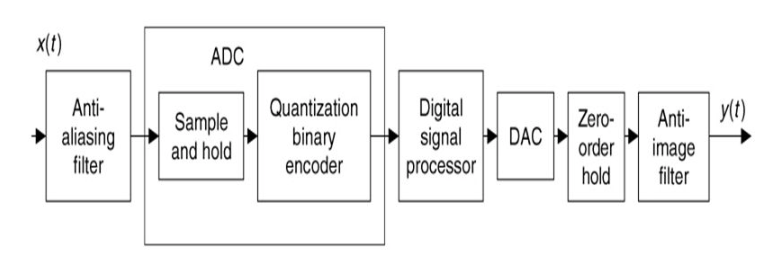
\includegraphics[width=0.8\textwidth]{grafer/Opgave1}
\caption{Et DSP system} \label{Opgave1}
\end{figure}

Det grundlæggende koncept for et DSP-system er illustreret på ovenstående figur \ref{Opgave1}. Systemet består af forskellige dele, hvor et inputsignal, x(t), betragtes. Den første box er det såkaldte ikke-ideele "anti-aliaserings lavpasfilter", hvor indgangssignalets lave frekvenser kommer igennem filtret, hvorimod de høje frekvenser, som overstiger Nyquist-kriteriet, dæmpes. Et ideelt "anti-aliaserings filter" fjerner alle de uønskede frekvenser og lader kun de relevante input frekvenser igennem. Det er dog ikke muligt, at have et ideelt "anti-aliaserings filter". 

Den næste box i DSP systemet er en AD-konvertering (ADC). I denne sker først en "sample and hold", der låser de analoge værdier på et konstant niveau i en bestemt tidsperiode, hvilket giver os et trappe lignende signal. Efterfølgende skal disse værdier igennem  "quantization binary encoder", som tager det analoge signal og kvantiserer dette til digitale værdier.

Næste box i DSP systemet er "digital signal processor" (DS), hvis opgave er at behandler det nu digitale signal.

Efter dette, skal det digitale signal konverteres tilbage til et analogt signal, hvor der anvendes en DA-konvertering (DAC). 
"Zero-order hold" udfører præcis samme funktion som "sample and hold", som også holder fast i den analoge værdi på et konstant niveau i en bestemt tidsperiode, hvilket giver os et trappe lignende signal.  

Den sidste del af DSP-systemet er "anti-image filtret". Dette filter udglatter de trappetrins lignende værdier, således at kurven bliver gjort pæn og brugbar, så det ligner input-signalet mest muligt.\\
\\

\section*{Opgave 1: Lavpas-filter til støjreduktion (fjern noget hvid-støj fra et talesignal)}
\textit{Indspil selv et talesignal i Matlab og tilføj efterfølgende hvid støj til signalet i Matlab.\\ 
Analyser signalet før og efter tilføjelse af hvid støj – og bestem de nødvendige filterspecifikationer til et lavpas-filter, så kun de absolut nødvendige talesignaler (med støj oveni) kommer igennem filteret.
Analyser signalet igen efter filtrering.}\\

Hvid støj defineres som et støjsignal hvor alle frekvenser repræsenteres med samme effekt. Ægte hvid støj er et uendeligt signal, der går fra tiden minus uendelig til plus uendelig med en uendelig samplingsfrekvens. I praksis er dette ikke muligt, og man arbejder derfor kun med et endeligt tidsdomæne hvor signalet har en begrænset båndbredde til den halve samplingsfrekvens (Nyquist). 


Koden er rettet til, således et menneske kan sige den samme søtning på omkring 5 sejunder. - sætningen lød: "Hvis jeg bliver mere klar, så bliver jeg sgu gennemsigtig!". 

Herunder ses talesignallet, hvor der er vist tidsdomæne, frekvensdomæne og henholdsvis to spektogrammer, med og uden hvid støj.

\begin{figure}[H] 
\centering
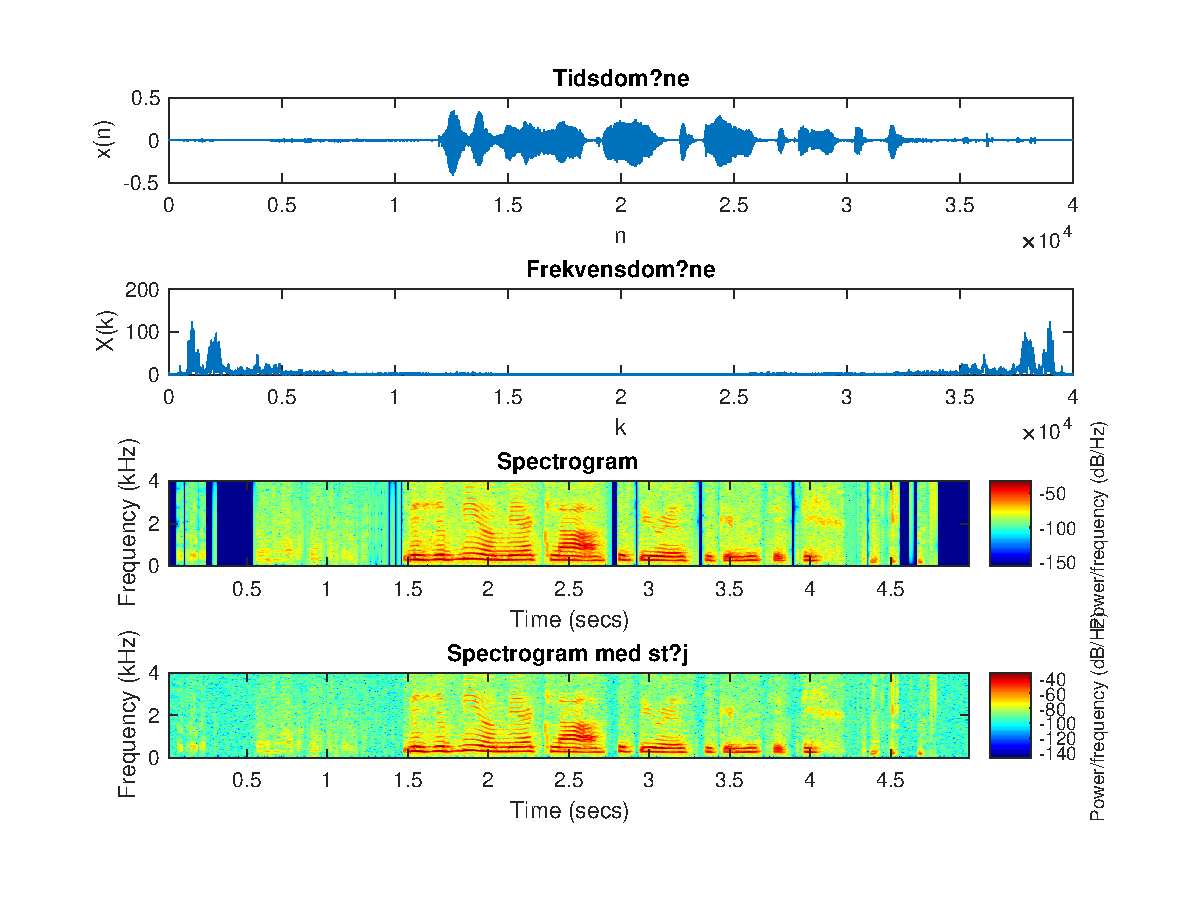
\includegraphics[width=0.7\textwidth]{grafer/White_noise_60}
\caption{Talesignal ved forskellige tilstande} \label{White_noise_60}
\end{figure}

(Teori om SNR, da vi har brugt awgn(x,SNR)) 

"Signal-støj-forhold (forkortet SNR eller S / N) er en foranstaltning, der anvendes inden for videnskab og teknik, som sammenligner niveauet af et ønsket signal til niveauet af baggrundsstøj. Det defineres som forholdet mellem signaleffekt til støjeffekten, ofte udtrykt i decibel. Et forhold større end 1: 1 (større end 0 dB) angiver mere signal end støj. Mens SNR er almindeligt citeret for elektriske signaler, kan den anvendes til enhver form for signal (såsom isotop niveauer i en iskerne eller biokemisk signalering mellem celler)."  

Evt. vis SNR. 


Herefter lavede vi et lavpasfilter vha. fdatool i Matlab. - vi valgte at generere et 8. ordens lavpas Fir filter, hvor samplingsfrekvensen er på 8000. Dette ses nedenfor. 

\begin{figure}[H] 
\centering
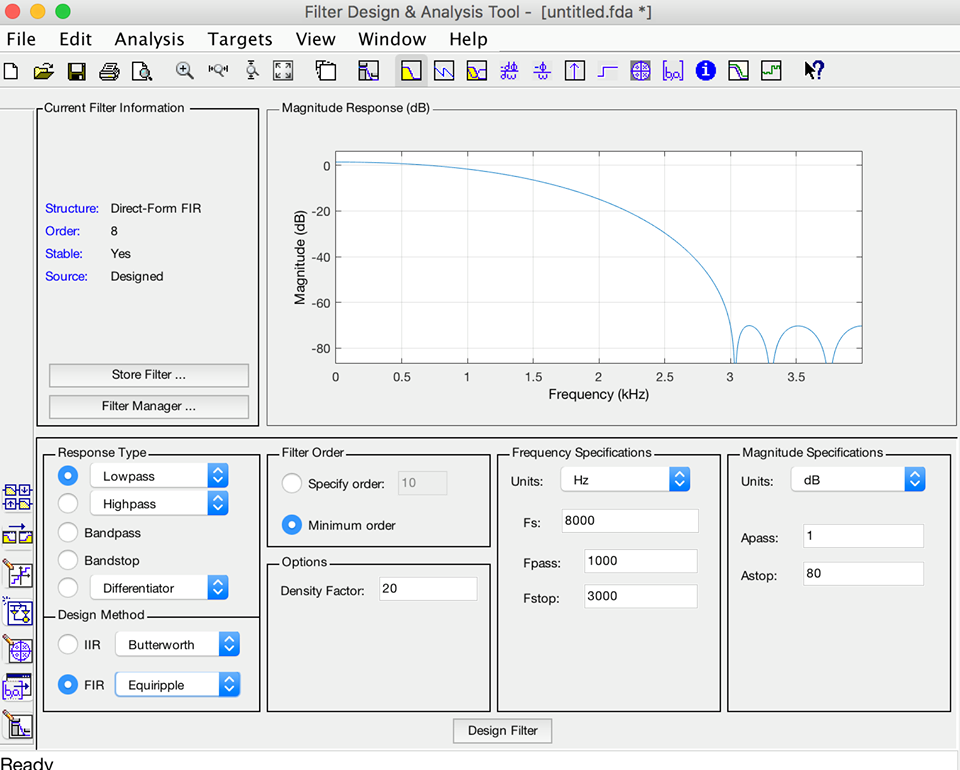
\includegraphics[width=0.7\textwidth]{grafer/lavpasfilter}
\caption{Talesignal ved forskellige tilstande} \label{lavpasfilter}
\end{figure}


For at køre talesignalet med hvis støj igennem vores lavpasfilter, gemte vi blot filterkoeficienterne fr fdatool i workspace. 

Herunder ses talesignalet efter filteringen: 

\begin{figure}[H] 
\centering
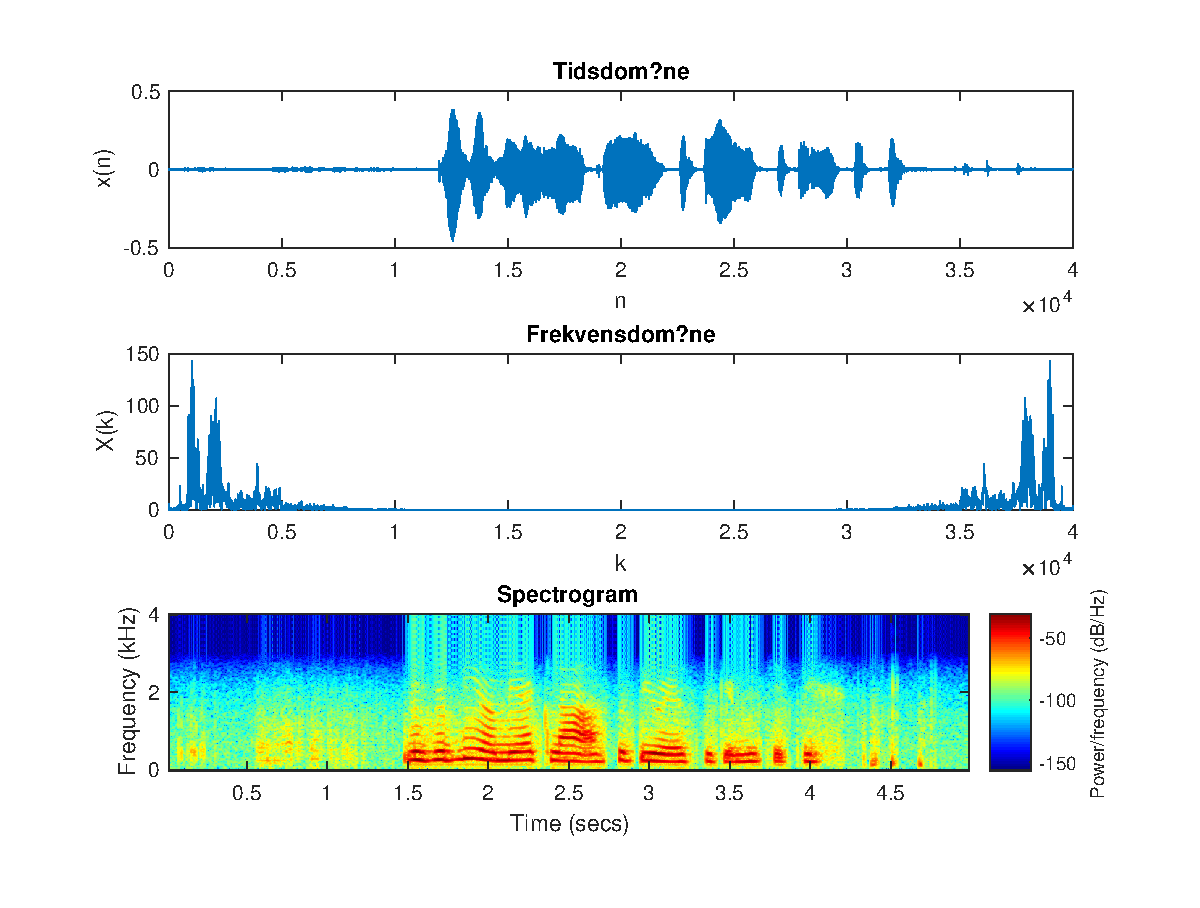
\includegraphics[width=0.7\textwidth]{grafer/opg1_filter}
\caption{Talesignal ved forskellige tilstande} \label{opg1_filter}
\end{figure}


Det er blåt, fordi støjen er fjernet.


\section*{Opgave 2: Båndpas-filter til analyse af vokaler ’a’  ’e’  ’i}
\textit{Indspil selv lyd som indeholder vokalerne ’a’  ’e’  ’i’ – analyser signalerne og bestem de nødvendige filterspecifikationer så f.eks. et ’a’ detekteres i ’en talestrøm’. Implementer filteret i Matlab og dokumenter designet.}\\


vi har valgt at indspille de 3 vokaler: 

et a: 

et e: 

et i: 





alle 3 signaler i en: 


\begin{figure}[H] 
\centering
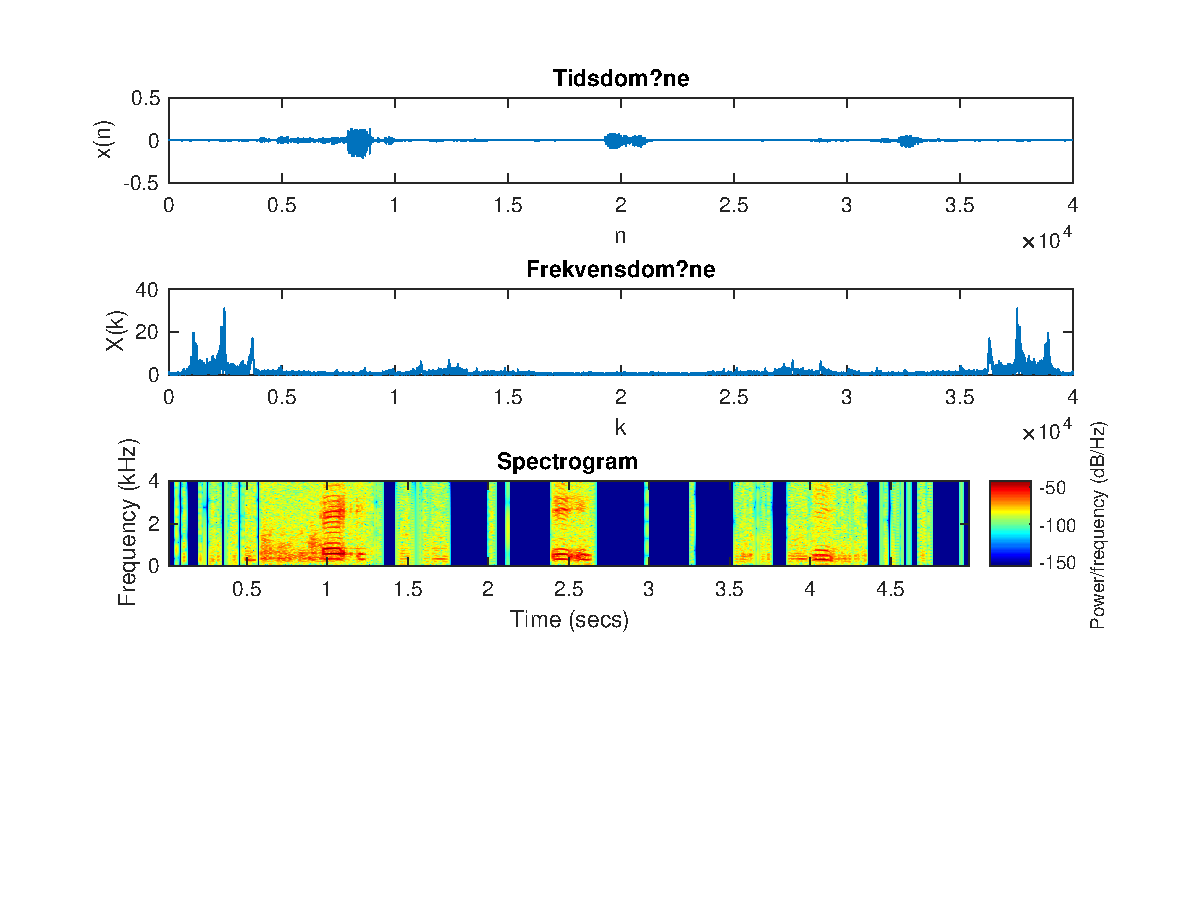
\includegraphics[width=0.7\textwidth]{grafer/opg2_vokaler}
\caption{Talesignal ved forskellige tilstande} \label{opg2_vokaler}
\end{figure}



\section*{Opgave 3: Båndstop filter til fjernelse af brumsignal}

\textit{I folderen '(Signaler til opgave3') ligger et signal med indlejret brum. Analyser signalet og bestem de nødvendige filterspecifikationer så brummen fjernes.Implementer filteret i Matlab og dokumenter designet}\\

\section*{Opgave 4: Filter til at finde triggerpunkt for EKG signal (ekg signal fra øvelse 1)}
\textit{Anvendt EKG signalet fra øvelse 1 – og proces signalet gennem en simpel  differentiering, så man kan finde et passende ’triggerpunkt’ til at bestemme bestemte steder på signalet. Implementer filteret i Matlab og dokumenter designet.}\\

\section*{Opgave 4: Filter til at finde triggerpunkt for EKG signal (ekg signal fra øvelse 1)}
\textit{Anvendt EKG signalet fra øvelse 1 – og proces signalet gennem en simpel  differentiering, så man kan finde et passende ’triggerpunkt’ til at bestemme bestemte steder på signalet. Implementer filteret i Matlab og dokumenter designet.
}\\

\section*{Opgave 5: Anvend en vindue-funktion på et af ovenstående signaler. Forklar hvorfor en vindue-funktion kan være nødvendig, hvad den gør og hvordan den anvendes.}
\textit{Vis ved et eksempel}\\

\end{document}




(Type your content here.)
\end{document}